\section{The Emergence of Legal Retrieval-Augmented Generation (2024)}
\label{sec:rag2024}

Four years after \citet{lewis2020} introduced retrieval-augmented generation for general-domain
tasks, and one year after \citet{guha2023} showed that benchmark success does not guarantee legal
reliability, 2024 was the year the field connected these two threads explicitly. This section
follows five studies published that year, in sequence. Each one addresses a different part of the
same emerging problem: how to retrieve legal evidence well, and how to know whether a generated
legal answer can be trusted.

\subsection{Evaluating legal case retrieval on its own terms}

\citet{feng2024} opened the year with a systematic survey of legal case retrieval. They pulled a
decade of scattered work, including the specialized datasets and models this survey has mentioned
only briefly so far, into a single account of the problem's defining feature. A relevant precedent
is not necessarily one that discusses the same topic. Its value depends on the similarity of the
legally material facts, the legal issue, the reasoning, and the outcome. That makes it a
substantially harder retrieval target than general-purpose document similarity.

\subsection{The hallucination problem becomes impossible to ignore}

\citet{dahl2024} then documented, empirically and at scale, a problem this survey has been building
toward since Section~\ref{sec:lm2023}. Large language models asked general-purpose legal questions
frequently invent authorities that do not exist, a phenomenon they call legal hallucination. Their
findings matter for a specific reason: a fluent, confident, well-formatted legal answer provides no
evidence, on its own, that it is correct. This is precisely the gap retrieval-augmented generation
is meant to close, by forcing a model to condition its answer on real, inspectable documents. Did it
actually close that gap? That was still an open empirical question for law specifically, and it is
exactly what the remaining 2024 studies, and much of Section~\ref{sec:reliability} later in this
survey, investigate.

\subsection{Evaluating retrieval itself, not just the final answer}

\citet{pipitone2024} addressed a specific weakness in how researchers were evaluating legal RAG.
Most existing benchmarks checked whether a system retrieved the correct \emph{document}, without
checking whether it retrieved the correct \emph{passage} within that document. Their benchmark,
\textbf{LegalBench-RAG}, evaluates retrieval of precise legal text segments rather than whole
documents. This matters because a document can be hundreds of pages long while only one paragraph
actually supports a given answer. Document-level retrieval can look successful while still failing
to surface the evidence a generator needs. In the same year, \citet{wiggers2024} proposed
\textbf{LeReRAG}, a method for measuring legal relevance specifically within retrieval-augmented
generation pipelines. It reinforces, from a different angle, the same conclusion: relevance, in a
legal setting, is a more demanding and more specific property than topical similarity. Finally,
\citet{goebel2024} published a second, extended overview of the 2023 COLIEE competition first
summarized by \citet{goebel2023} the previous year, continuing the benchmark series this survey
revisits once more in Section~\ref{sec:2026}.

\subsection{The retrieval techniques these systems actually use}

This year's five studies now define the problem well, so it helps to describe, in one place, the
retrieval techniques the legal RAG systems discussed throughout the rest of this survey actually
build on. \textbf{Lexical retrieval}, typically implemented with the BM25 ranking function, scores
passages by term frequency and specificity. It suits the highly specific expressions common in
legal queries, such as section numbers and defined terms, but it can miss relevant evidence when a
question and its authority use different wording. \textbf{Dense retrieval} represents queries and
documents as embedding vectors and retrieves by similarity, which responds to conceptual overlap
regardless of wording. But semantic similarity is not legal relevance, as \citet{feng2024} and
\citet{wiggers2024} both point out. A judgment may discuss a doctrine while rejecting its
applicability to the facts, and a dense retriever can still rank such material highly.
\textbf{Hybrid retrieval} combines both signals, commonly through the Reciprocal Rank Fusion method
\citet{cormack2009} introduced outside the legal domain, back in Section~\ref{sec:foundations}.
Fifteen years later, it is exactly this kind of legal hybrid-retrieval problem that gives RRF its
legal relevance. Fusion combines rankings; it does not independently verify legal correctness. If
every retrieval stream returns irrelevant evidence, fusion cannot turn that evidence into
authoritative support.

Beyond combining retrieval methods, legal documents also need \textbf{structure-aware indexing}.
Conventional chunking divides documents by a fixed token limit or text boundary, which can separate
a provision from its heading, its parent section, or an exception that qualifies it. A query that
retrieves only a general rule may miss the proviso that changes its application. Structure-aware
indexing cuts this risk by keeping hierarchical breadcrumbs, section identifiers, and parent-child
relationships alongside the text. \textbf{Knowledge-graph retrieval}, building on the graph-based
systems \citet{sovrano2020} and \citet{zhu2022} introduced in Section~\ref{sec:lm2023}, offers a
complementary representation across documents instead of within one. It encodes legal entities,
such as statutes, provisions, cases, and courts, as nodes. It encodes relationships, such as
interpretation, amendment, and citation, as edges. This can support retrieval beyond direct text
similarity, moving from a provision to the judgments that interpret it. Graph quality, however,
depends entirely on the accuracy of entity extraction and relationship identification. A graph that
records a judgment citing a provision does not mean the judgment adopts or endorses that provision's
interpretation.

\subsection{A unified retrieval architecture}

These techniques address different parts of the retrieval problem. We can organize them as a single
staged pipeline, shown in Figure~\ref{fig:arch}. Structure-aware preprocessing feeds parallel
lexical and dense retrieval. Rank fusion and reranking combine their results. The system then checks
those results against parent provisions and jurisdictional context, and finally uses them for
evidence-grounded generation and verification. A knowledge graph can attach at the
context-and-authority stage, and an agentic controller can trigger additional retrieval when
evidence is incomplete, though measurable benefit should justify both additions rather than
complexity for its own sake. This is our own synthesis of the preceding techniques, not an
architecture any single cited study proposed.

% Conceptual unified legal retrieval architecture (horizontal pipeline, full page width).
\begin{figure*}[t]
\centering
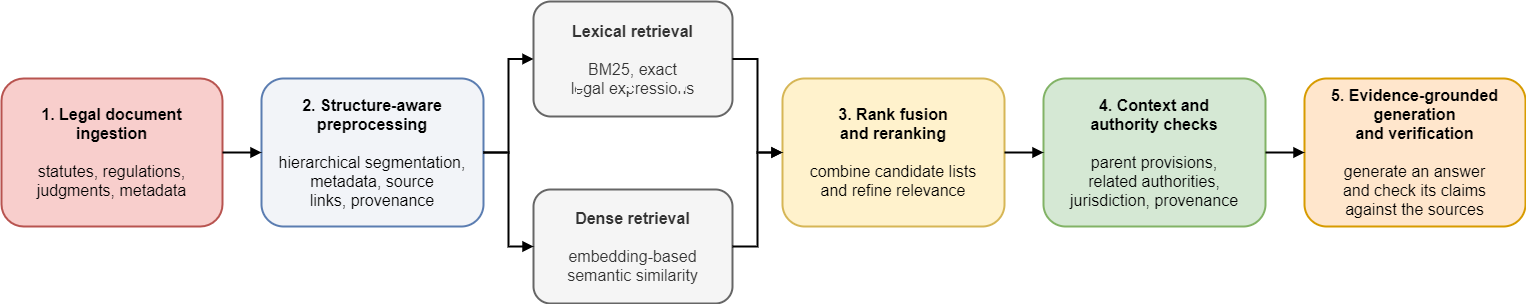
\includegraphics[width=\textwidth]{images/legal_rag_pipeline.png}
\caption{Conceptual architecture synthesizing complementary legal retrieval methods. This is a
proposed reference architecture, not a claim that every component has been validated together in a
single experiment.}
\label{fig:arch}
\end{figure*}


\subsection{Evaluating retrieval and RAG architectures}

We should assess a retrieval architecture independently of the quality of its generated answers.
The generator cannot reliably make up for evidence the retriever failed to return, and successful
retrieval does not establish that the generator interprets that evidence correctly.
Table~\ref{tab:metrics} summarizes the complementary metrics this requires, drawing on the
retrieval and evaluation literature this section discusses.

\begin{table*}[tp]
\centering
\caption{Complementary metrics for evaluating legal retrieval and RAG architectures.}
\label{tab:metrics}
\footnotesize
\setlength{\tabcolsep}{5pt}
\renewcommand{\arraystretch}{1.25}
\begin{tabularx}{\textwidth}{>{\raggedright\arraybackslash}p{4.0cm} >{\raggedright\arraybackslash}X >{\raggedright\arraybackslash}X}
\toprule
\textbf{Metric} & \textbf{What it measures} & \textbf{Why it matters in legal retrieval} \\
\midrule
Recall@$k$ / Precision@$k$ & Whether, and how purely, relevant evidence appears among the top $k$ results. & Finds needed authorities while bounding irrelevant material entering generation. \\
MRR / nDCG & How early a relevant result appears, and ranking quality under graded relevance. & Distinguishes highly relevant legal evidence from merely related passages. \\
Passage-level retrieval accuracy & Whether a system retrieved the specific supporting passage, not just the document \citep{pipitone2024}. & A correct document with the wrong passage still fails to support a generated answer. \\
Citation precision / recall & Proportion of citations that correctly support their claim, and of required support that is cited. & Measures whether references are evidentially useful and whether support is missing. \\
Unsupported-claim rate & Proportion of evaluated claims lacking adequate support in the permitted evidence. & Evaluates grounding beyond the mere presence of citations. \\
\bottomrule
\end{tabularx}
\end{table*}

These metrics need explicit annotation guidelines. Relevance can be graded at the document or
passage level with different results, and citation correctness needs a stated definition of what
counts as support. None of the architectural components this section discusses independently
guarantees legal correctness; their value depends on the corpus, provenance, and evaluation
protocol. The following year, 2025, is where the field put these retrieval techniques and evaluation
metrics to work in complete, deployed legal RAG systems, which Section~\ref{sec:maturing} takes up
next.
